%% Fig. 1 overview for
%% "Transfer-Learning Surrogates for Scalable Multi-Fidelity Bayesian Optimization in Molecular and Materials Discovery"
%% Vector source of paper_figures/fig1_overview.pdf (3-panel schematic); labels match the main text
%% (DKL; up to 22x fewer FLOPs, BLR-head profile 2026-09-14). Edited 2026-09-03 for the NCS submission:
%% panels widened and shortened so the content fills them, fonts one step larger, included at \textwidth.
%% Counts updated 2026-09-14 to the final data basis (13 benchmarks; 3 GP + 5 TL surrogates: NARGP excluded;
%% Sequential, Progressive, feature-extraction transfer (Curriculum/KD/Pseudo-labelling) and Adapter dropped, leaving
%% Frozen-representation transfer, Pretrain-then-Joint, End-to-End Joint, Soft Parameter Sharing and Domain Adaptation
%% (MMD)). 2026-09-17: the "TL-base >= GP-base on all 9 molecular & materials pools" line under the regret sketch was removed
%% (author decision); the panel letter is no longer overlaid in LaTeX text but included as paper_figures/fig1_letter_a.pdf
%% (DejaVu Sans Bold, the glyph of the b-p letters).
%% Helvetica, colour-blind-safe blue/orange palette (matches graphical_abstract.tex / Figs 2-4).
%% Build:  pdflatex fig1_overview.tex  ->  fig1_overview.pdf (auto-cropped)
\documentclass[border=6pt]{standalone}
\usepackage[T1]{fontenc}
\usepackage{helvet}
\renewcommand{\familydefault}{\sfdefault}
\usepackage{amsmath}
\usepackage{tikz}
\usetikzlibrary{arrows.meta,positioning,fit,calc}

% ---- palette (matches graphical_abstract.tex / Figs 2-4) ----
\definecolor{gpcol}{RGB}{242,170,132}   % salmon (light)  -- GP
\definecolor{gpbox}{RGB}{199,109,63}    % GP family box (orange)
\definecolor{tlcol}{RGB}{78,149,217}    % blue (light)    -- TL
\definecolor{tlbox}{RGB}{60,110,180}    % TL box (blue)
\definecolor{tldk}{RGB}{38,92,148}
\definecolor{navy}{RGB}{31,78,128}      % flask
\definecolor{ink}{RGB}{43,50,64}
\definecolor{sub}{RGB}{120,130,144}
\definecolor{pline}{RGB}{208,214,223}

\begin{document}
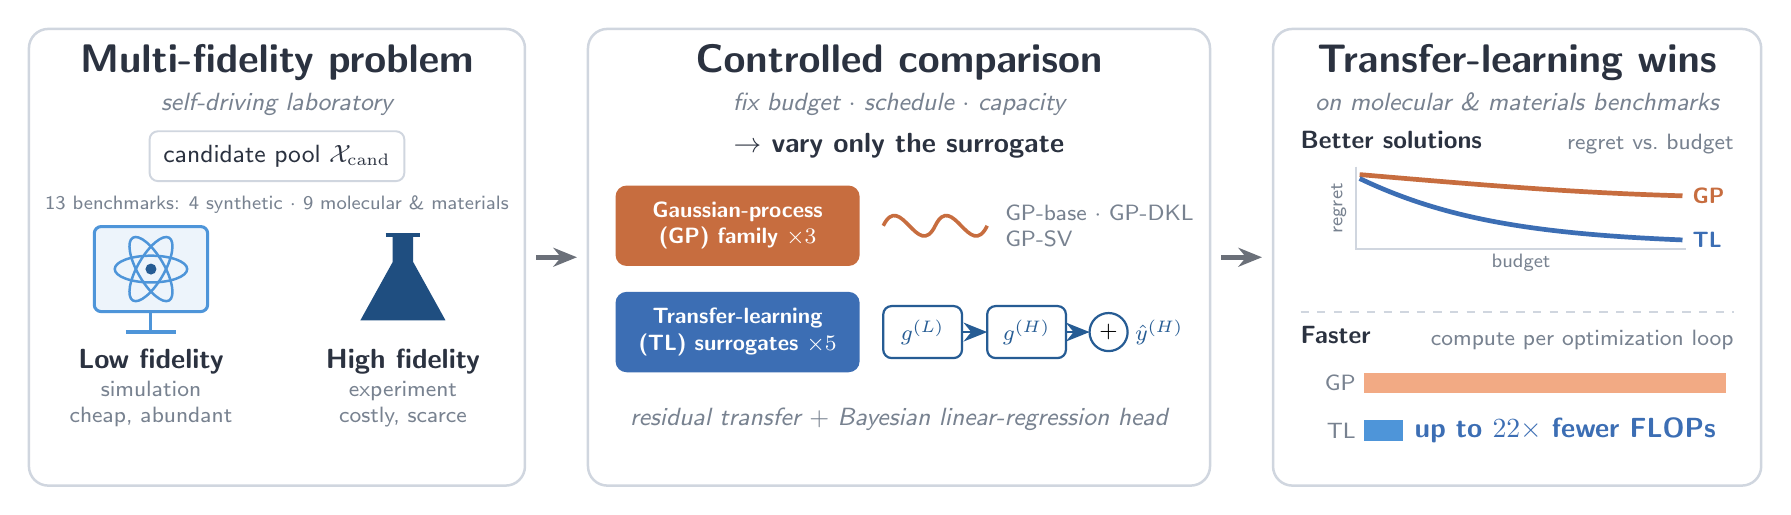
\begin{tikzpicture}[
  font=\sffamily,
  >={Stealth[length=3mm,width=2.4mm]},
  every node/.style={inner sep=0pt, outer sep=0pt},
  panelbox/.style={rounded corners=7pt, draw=pline, line width=0.9pt, fill=white},
  hdr/.style={text=ink, font=\bfseries\Large, align=center},
  slab/.style={text=sub, font=\small\itshape, align=center},
  blab/.style={text=ink, font=\bfseries\normalsize, align=center},
  glab/.style={text=sub, font=\footnotesize, align=left},
  chip/.style={rounded corners=4pt, inner xsep=6pt, inner ysep=6pt, minimum width=3.1cm,
               font=\bfseries\footnotesize, text=white, align=center},
  netbox/.style={rounded corners=3pt, draw=tldk, line width=0.8pt, fill=white,
                 minimum width=1.0cm, minimum height=0.66cm, font=\footnotesize, text=tldk, align=center},
  pflow/.style={->, line width=1.8pt, draw=ink!70},
]

% ===== panel geometry (22 cm wide, 5.8 cm tall; included at \textwidth = 16 cm) =====
\def\ya{0}\def\yb{5.8}
\def\Al{0}\def\Ar{6.3}
\def\Bl{7.1}\def\Brr{15.0}
\def\Cl{15.8}\def\Cr{22.0}
\pgfmathsetmacro\Ac{(\Al+\Ar)/2}
\pgfmathsetmacro\Bc{(\Bl+\Brr)/2}
\pgfmathsetmacro\Cc{(\Cl+\Cr)/2}
\pgfmathsetmacro\ymid{(\ya+\yb)/2}

% ===================== PANEL A : multi-fidelity problem =====================
\node[panelbox, fit={(\Al,\ya) (\Ar,\yb)}] (PA) {};
\node[hdr, anchor=north] at (\Ac,\yb-0.20) {Multi-fidelity problem};
\node[slab, anchor=north] at (\Ac,\yb-0.82) {self-driving laboratory};
\node[text=ink, font=\small, draw=pline, line width=0.7pt, rounded corners=3pt, fill=white,
      inner sep=5pt, anchor=north] at (\Ac,\yb-1.30) {candidate pool $\mathcal{X}_{\mathrm{cand}}$};
\node[text=sub, font=\scriptsize, anchor=north, align=center] at (\Ac,\yb-2.12)
     {13 benchmarks: 4 synthetic $\cdot$ 9 molecular \& materials};

% --- monitor icon (LF) ---
\pgfmathsetmacro\mx{1.55}\pgfmathsetmacro\my{2.75}
\draw[tlcol, line width=1.1pt, fill=tlcol!10, rounded corners=2.5pt]
      (\mx-0.72,\my-0.54) rectangle (\mx+0.72,\my+0.54);
\draw[tlcol, line width=1.1pt] (\mx,\my-0.54)--(\mx,\my-0.80);
\draw[tlcol, line width=1.6pt] (\mx-0.32,\my-0.80)--(\mx+0.32,\my-0.80);
\foreach \a in {0,60,120}{
  \draw[tlcol, line width=0.9pt, rotate around={\a:(\mx,\my)}] (\mx,\my) ellipse (0.46 and 0.17);}
\fill[tldk] (\mx,\my) circle (0.07);
\node[blab, anchor=north] at (\mx,\my-1.02) {Low fidelity};
\node[text=sub, font=\footnotesize, anchor=north, align=center] at (\mx,\my-1.42)
     {simulation\\cheap, abundant};

% --- flask icon (HF) ---
\pgfmathsetmacro\fx{4.75}\pgfmathsetmacro\fy{2.66}
\fill[navy] (\fx-0.13,\fy+0.52) -- (\fx-0.13,\fy+0.18) -- (\fx-0.54,\fy-0.56)
            -- (\fx+0.54,\fy-0.56) -- (\fx+0.13,\fy+0.18) -- (\fx+0.13,\fy+0.52) -- cycle;
\draw[navy, line width=1.5pt] (\fx-0.22,\fy+0.52)--(\fx+0.22,\fy+0.52);
\node[blab, anchor=north] at (\fx,\fy-0.93) {High fidelity};
\node[text=sub, font=\footnotesize, anchor=north, align=center] at (\fx,\fy-1.33)
     {experiment\\costly, scarce};

% ===================== arrow A -> B =====================
\draw[pflow] (\Ar+0.14,\ymid) -- (\Bl-0.14,\ymid);

% ===================== PANEL B : controlled comparison =====================
\node[panelbox, fit={(\Bl,\ya) (\Brr,\yb)}] (PB) {};
\node[hdr, anchor=north] at (\Bc,\yb-0.20) {Controlled comparison};
\node[slab, anchor=north] at (\Bc,\yb-0.82) {fix budget $\cdot$ schedule $\cdot$ capacity};
\node[blab, anchor=north] at (\Bc,\yb-1.32) {$\rightarrow$ vary only the surrogate};

% GP lane
\node[chip, fill=gpbox, anchor=west] (gpc) at (\Bl+0.35,3.3)
     {Gaussian-process\\(GP) family $\times 3$};
\draw[gpbox, line width=1.3pt]
   (10.85,3.3) .. controls (11.07,3.75) and (11.29,2.85) .. (11.51,3.3)
   .. controls (11.73,3.75) and (11.95,2.85) .. (12.17,3.3);
\node[glab, anchor=west] at (12.4,3.3) {GP-base $\cdot$ GP-DKL\\GP-SV};

% TL lane
\node[chip, fill=tlbox, anchor=west] (tlc) at (\Bl+0.35,1.95)
     {Transfer-learning\\(TL) surrogates $\times 5$};
\node[netbox, anchor=west] (gL) at (10.85,1.95) {$g^{(L)}$};
\node[netbox, right=0.32cm of gL] (gH) {$g^{(H)}$};
\node[circle, draw=tldk, line width=0.8pt, fill=white, inner sep=1.8pt, font=\footnotesize,
      right=0.30cm of gH] (sm) {$+$};
\draw[->,line width=0.8pt,draw=tldk] (gL)--(gH);
\draw[->,line width=0.8pt,draw=tldk] (gH)--(sm);
\node[text=tldk, font=\footnotesize, anchor=west] at ($(sm.east)+(0.1,0)$) {$\hat{y}^{(H)}$};

\node[slab, anchor=north] at (\Bc,0.98) {residual transfer $+$ Bayesian linear-regression head};

% ===================== arrow B -> C =====================
\draw[pflow] (\Brr+0.14,\ymid) -- (\Cl-0.14,\ymid);

% ===================== PANEL C : transfer-learning wins =====================
\node[panelbox, fit={(\Cl,\ya) (\Cr,\yb)}] (PC) {};
\node[hdr, anchor=north] at (\Cc,\yb-0.20) {Transfer-learning wins};
\node[slab, anchor=north] at (\Cc,\yb-0.82) {on molecular \& materials benchmarks};

% ---- zone 1 : better solutions ----
\node[text=ink, font=\bfseries\small, anchor=north west] at (\Cl+0.35,\yb-1.30) {Better solutions};
\node[text=sub, font=\footnotesize, anchor=north east] at (\Cr-0.35,\yb-1.34) {regret vs.\ budget};
\begin{scope}[shift={(\Cl+1.05,3.0)}]
  \draw[pline, line width=0.8pt] (0,1.05) -- (0,0) -- (4.2,0);
  \node[text=sub, font=\scriptsize, anchor=south, rotate=90] at (-0.12,0.52) {regret};
  \node[text=sub, font=\scriptsize, anchor=north] at (2.1,-0.06) {budget};
  \draw[gpbox, line width=1.7pt] (0.05,0.95) .. controls (1.8,0.8) and (2.8,0.72) .. (4.15,0.68);
  \draw[tlbox, line width=1.7pt] (0.05,0.9) .. controls (1.1,0.4) and (2.2,0.2) .. (4.15,0.12);
  \node[text=gpbox, font=\footnotesize\bfseries, anchor=west] at (4.28,0.68) {GP};
  \node[text=tlbox, font=\footnotesize\bfseries, anchor=west] at (4.28,0.12) {TL};
\end{scope}

% ---- divider ----
\draw[pline, line width=0.8pt, dashed] (\Cl+0.35,2.2) -- (\Cr-0.35,2.2);

% ---- zone 2 : faster ----
\node[text=ink, font=\bfseries\small, anchor=north west] at (\Cl+0.35,2.02) {Faster};
\node[text=sub, font=\footnotesize, anchor=north east] at (\Cr-0.35,1.98) {compute per optimization loop};
\node[glab, anchor=east, text=sub] at (\Cl+1.05,1.30) {GP};
\fill[gpcol] (\Cl+1.15,1.17) rectangle (\Cr-0.45,1.43);
\node[glab, anchor=east, text=sub] at (\Cl+1.05,0.70) {TL};
\fill[tlcol] (\Cl+1.15,0.57) rectangle (\Cl+1.65,0.83);
\node[text=tlbox, font=\bfseries\normalsize, anchor=west] at (\Cl+1.8,0.70) {up to $22\times$ fewer FLOPs};

\end{tikzpicture}
\end{document}
